\section{平面图}
\subsection{平面图的性质和概念}
\begin{definition}
如果能把图$G$画在平面上,使得除顶点外,\textcolor{red}{边与边
之间没有交叉},称$G$可以嵌入平面,或称$G$是\colorbox{yellow}{\textcolor{red}{可平面图}}. 可
平面图$G$的边不交叉的一种画法,称为$G$的一种平面嵌入,
G的平面嵌入表示的图称为\colorbox{yellow}{\textcolor{red}{平面图}}.
\end{definition}

\begin{definition}
一个平面图$G$把平面分成若干连通片,这些连
通片称为$G$的区域,或$G$的一个面. $G$的面组成的集合用\colorbox{yellow}{$\phi$}表示. 面积有限的区域称为平面图$G$的内部面,否则称为$G$
的外部面. 某面$f$ 的边界中含有的边数(\textcolor{red}{割边计算2次})
称为该面\colorbox{yellow}{\textcolor{red}{$f$ 的次数}}, 记为\colorbox{yellow}{$deg (f)$}.
\end{definition}
\begin{note}
	\begin{enumerate}
		\item \textcolor{red}{平面图外部面只有一个}.
		\item 可以把平面图的任意一个内部面转换为外部面.
	\end{enumerate}
	
\end{note}

\begin{theorem}[次数公式]
	设$G=(n, m)$是平面图,则:
	\colorbox{yellow}{$\sum\limits_{f \in \phi} deg(f) = 2m$}.
\end{theorem}
\begin{theorem}[欧拉公式]
	\label{oula}
	设$G=(n, m)$是连通平面图,$\phi$是$G$的面数,则:
	\colorbox{yellow}{$n-m+\phi =2$}.
\end{theorem}
\begin{corollary}
	\label{tuilun}
	\begin{enumerate}
		\item 设$G$是具有$\phi $个面$k$个连通分支的平面图,则:
		\[
		\colorbox{yellow}{$n-m+\phi =k+1$}
		\]
		\begin{proof}
			对第$i (1\leq i\leq k  )$个分支来说,设顶点数为$n_i$,边数
			为$m_i$,面数为$\phi_i$,由欧拉公式:$n_i-m_i+\phi_i =2 \Rightarrow \sum\limits_{i=1}^k(n_i-m_i+\phi_i)=2k$,又$\sum\limits_{i=1}^kn_i=n,\sum\limits_{i=1}^km_i=m, \sum\limits_{i=1}^k\phi_i=\phi+k-1$,故得$n-m+\phi =k+1$.
		\end{proof}
		\item \label{hhbggg}设$G=(n, m)$是连通平面图,$\phi$是$G$的面数,如
		果对$G$的每个面$f$ ,有:$deg (f) \geq l \geq 3$,则:
			\[
		\colorbox{yellow}{$m\leq \dfrac{l}{l-2}(n-2)$}
		\]
		\begin{proof}
			由次数公式得:
			$\sum\limits_{f \in \phi} deg(f) = 2m\geq \phi l\Rightarrow \phi \leq \frac{2m}{l}$. 由欧拉公式得:$\phi = 2+m-n\leq \frac{2m}{l} \Rightarrow m\leq \dfrac{l}{l-2}(n-2)$.
		\end{proof}
		\begin{note}
			推论\ref{hhbggg}得不等式条件是必要非充分的,其等价说法为:
			
			设$G=(n, m)$是连通图,如果\colorbox{yellow}{$m> \frac{l}{l-2}(n-2)$},则$G$是非可平面图(\textcolor{red}{常用}).
		\end{note}
		\item \label{hhhhhkkgga}设$G$是具有$n$个点$m$条边$\phi$个面的简单可平面图,若$n\geq 3$,则:\colorbox{yellow}{$m\leq 3n-6$}.
			\begin{note}
		如果\colorbox{yellow}{$m> 3n-6$},则$G$是非可平面图. $K_{3,3}$ 是非可平面图,$K_5$ 是非可平面图.
		\end{note}
		\item 设$G$是具有$n$个点$m$条边的连通平面图,若$G$的
		每个圈均由长度是$l$的圈围成,则:
		\colorbox{yellow}{$m(l-2)=l(n-2)$}
		\begin{proof}
	将推论\ref{hhbggg}的证明中的符号改成等号.
		\end{proof}
	\item 设$G$是具有$n$个点$m$条边的简单平面图,则:\colorbox{yellow}{$\delta \leq 5$}.
	\begin{proof}
		设$G$有$n$个顶点$m$条边. 对$n=1,2$经直接验证得结论成立. 假设$n\geq 3$,假设$\delta \geq 6$,则
		\[
		6n-12<6n \leq \sum\limits_{v\in V(G)}d(v) =2m \Rightarrow m> 3n-6
		\]故$G$是非可平面图,与原命题矛盾,假设不成立. 因此$\delta \leq 6$.
	\end{proof}

\end{enumerate}
\end{corollary}


\begin{theorem}
存在且只存在$5$种正多面体:它们是正四、六、
八、十二、二十面体.
\end{theorem}

\begin{example}
	证明:每个五连通简单可平面图至少有12个顶点.
\end{example}
\begin{proof}
	设该图为$G(n\geq 3)$.
	
	依题意可得:$\delta(G)\geq k(G)\geq 5$. 由握手定理可得: $2m=\sum\limits_{v\in V(G)}d(v)\geq 5n$
	
	又$G$是可平面图,故$m\leq 3n-6$.
	
	因此,$2.5n\leq m \leq 3n-6\Rightarrow n\geq 12$, 故图$G$至少有12个顶点.
\end{proof}


\begin{example}
	若 $G$ 是一个连通平面图且满足 $\delta\geq3$,则 $G$ 至少有一个面使得 $deg(f) \leq 5$.
\end{example}
\begin{proof}
	若不然,则$deg(f) \geq 6$.
	
	$2m=\sum\limits_{f } deg(f) \geq 6\phi \mbox{且} n-m+\phi = 2\Rightarrow 2m \leq  3n-6$.
	
	又因所有顶点度数不小于3,故由握手定理得$2m=\sum\limits_{v\in V(G)}d(v)\geq 3n>3n-6$. 得出矛盾!
\end{proof}
\begin{example}
	证明:在$n(n\geq 3)$阶简单平面图$G$中有$\phi \leq 2n-4$,这里$\phi$是面数.
\end{example}
\begin{proof}
显然,每个面次数$l\geq 3$,则$2m= \phi l\geq 3\phi $. 又$n-m+\phi = 2$,故$\phi \leq 2n-4$.
\end{proof}

\subsection{特殊平面图与平面图的对偶图}
\subsubsection{极大平面图}
\begin{definition}
设G是简单可平面图,如果$G$是$K_i(1\geq i \geq 4)$,或
者在G的任意非邻接顶点间添加一条边后,得到的图均是
非可平面图,则称$G$是\colorbox{yellow}{\textcolor{red}{极大可平面图}}. 极大可平面图的平面嵌入称为\colorbox{yellow}{\textcolor{red}{极大平面图}}.
\end{definition}
\begin{note}
	\textcolor{red}{只有在简单图前提下才能定义极大平面图}
\end{note}

\begin{lemma}
设$G$是极大平面图,则$G$必然连通;且若$G$的阶数
大于等于$3$,则$G$无割边.
\end{lemma}

\begin{theorem}
	\textcolor{red}{设$G$是至少有3个顶点的平面图,则$G$是极大平
	面图,当且仅当$G$的每个面的次数是$3$且为单图}.
\end{theorem}

\begin{corollary}
	设$G$是$n$个点,$m$条边和$\phi$个面的极大平面图,
且$n\geq 3$.则:

(1) \colorbox{yellow}{$m=3n-6$}; (2) \colorbox{yellow}{$\phi=2n-4$}.
\end{corollary}
\begin{proof}
	因为$G$是极大平面图,则每个面的次数$l =3$.由次数公式得:
	$2m = \sum\limits_{f \in \phi} deg(f)= 3\phi$. 由欧拉公式得:$\phi = 2-n+m\leq \frac{2m}{l}\Rightarrow \frac{2}{3} m=2-n+m\Rightarrow m = 3n-6$. 又$m=n+\phi -2$, 故$\phi=2n-4$.
\end{proof}
\begin{note}
	\textcolor{red}{顶点数相同得极大平面图并不唯一}.
\end{note}

\begin{definition}
	如果在不可平面图$G$中任意删去一条边所得的图
	为可平面图,则称$G$为\textcolor{red}{极小不可平面图}.
\end{definition}
\begin{note}
	$K_{3,3}$和$K_5$ 是极小不可平面图.
\end{note}



\subsubsection{外可平面图}
\begin{definition}
若一个可平面图$G$存在一种平面嵌入,使得其所
有顶点均在某个面的边界上,称该图为\textcolor{red}{外可平面图}. 外可
平面图的一种外平面嵌入,称为\textcolor{red}{外平面图}.


设$G$是一个简单外可平面图,若在G中任意不邻
接顶点间添上一条边后,$G$成为非外可平面图,则称$G$是
\colorbox{yellow}{\textcolor{red}{极大外可平面图}}. 极大外可平面图的外平面嵌入,称为\colorbox{yellow}{\textcolor{red}{极
大外平面图}}.
\end{definition}

\begin{example}
	设 \( G \) 是一个具有 \( n(n \geq 4) \) 个点, \( m \) 条边的简单连通外平面图. 若 \( G \) 不含三 角形, 则 \( m \leq(3 n-4) / 2 \).
	
	\noindent {\bfseries\songti \textcolor{ecolor}{解:}} 假设 \( G \) 的所有顶点在外部面的边界上, 则由条件知: \( G \) 的外部面的次数至少为 \( n \), 内部面的次数至少为 \( 4(G \) 不含三角形 \( ) \). 设 \( G \) 有 \( \phi \) 个面, 则 $2m \geq 4(\phi-1)+n$. 由欧拉公式得, $\phi=2-n+m$. 因此, 根据上述两式得\( m \leq(3 n-4) / 2 \).
\end{example}

\begin{lemma}
	设$G$是一个连通简单外可平面图,则在$G$中存
	在度数至多是2的顶点.
\end{lemma}
\begin{theorem}
设$G$是一个有$n (n\geq 3)$个点,$m$条边,且所有点均在外部面
上的极大外平面图,则$G$有\colorbox{yellow}{$n-2$}个内部面且$m=3(n-2)-(n-2-1)=2n-3$.
\end{theorem}

\begin{theorem}
设$G$是一个有$n (n\geq 3)$个点,且所有点均在外部面
上的外平面图,则$G$是极大外平面图,当且仅当其\colorbox{yellow}{\textcolor{red}{外部面
的边界是圈,内部面是三角形}}.
\end{theorem}

\begin{theorem}
每一个至少有7个顶点的外可平面图的补图不是外
可平面图,且7是这个数目的最小者($n=6$,外可平面图的补图也是外可平面图).
\end{theorem}



\subsubsection{平面图的对偶图}
\begin{definition}
	给定平面图$G$,$G$的对偶图$G^{*}$如下构造:
	\begin{enumerate}
		\item 在$G$的每个面$f_i$内取一个点$v_i^{*}$作为$G^{*}$的一个顶点;
		\item 对$G$的一条边$e$, 若$e$是面$f_i$ 与$f_j$ 的公共边,则连接$v_i^{*}$
		与$v_j^{*}$,且连线穿过边$e$;若$e$是面$f_i$ 中的割边,则以$v_i$为顶点
		作环,且让它与$e$相交.
	\end{enumerate}
\end{definition}
\begin{figure}[H]
	\small
	\centering 
	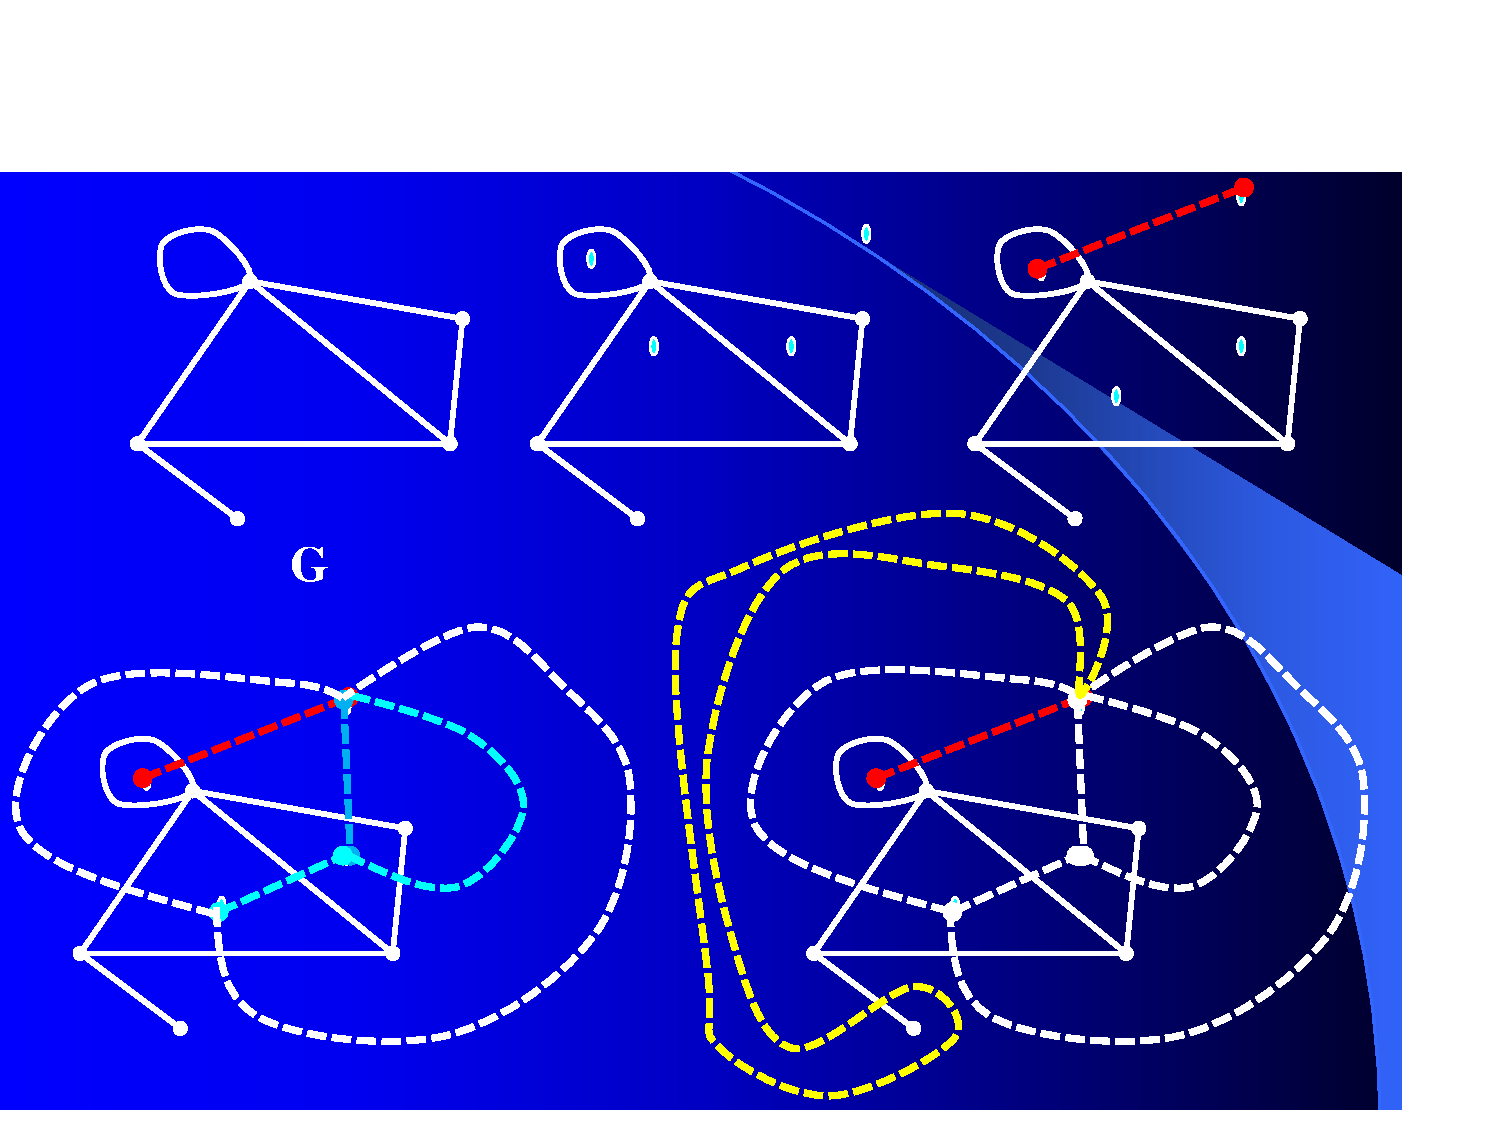
\includegraphics[scale=0.4]{image/CH6_duiou.pdf}  
	%\caption{信息包结构} 
	\label{fikgkjjj1Kjk}  
\end{figure}


\noindent \textcolor{ecolor}{\bfseries $G$与$G^{*}$的对应关系}
\begin{enumerate}
	\item $G^{*}$的顶点数$=G$的面数;
	\item $G^{*}$的边数$=G$的边数;
	\item $G^{*}$的面数$=G$的顶点数;
	\item $d(v^{*})=deg(f)$
\end{enumerate}
\begin{theorem}
平面图$G$的对偶图必然连通.
\end{theorem}
\begin{note}
	\begin{enumerate}
		\item $(G ^{*})^{*}$不一定等于$G$;
		\item $G$是平面图,则\colorbox{yellow}{$(G ^{*})^{*}\cong G$}当且仅当$G$是连通的;
		\item 同构的平面图可以有不同构的对偶图.
	\end{enumerate}
\end{note}
\begin{example}
	若平面图 $G$ 是自对偶的 $G\cong G ^{*}$,则 $m=2n-2$.
	
	\noindent {\bfseries\songti \textcolor{ecolor}{解:}} 设$G, G ^{*}$阶数分别为$n, n^{*}$,则必有$n=n^{*}$. 设$G$的面数为$\phi$,则$\phi=n^{*}$. $G ^{*}$连通$\Rightarrow G$连通. 由连通平面图欧拉公式,得:$2=n-m+\phi = n-m+n^{*}=n-m+n\Rightarrow m=2n-4$.
\end{example}




\subsection{平面图的判定}
之前平面图判定方法包括:\colorbox{yellow}{观察法、定理\ref{oula}(欧拉公式)推论\ref{hhbggg}和推论\ref{hhhhhkkgga}}


\begin{definition}
	两个图$G_1$与$G_2$,如果\colorbox{yellow}{$G_1\cong G_2$} ,或
	者通过反复在\colorbox{yellow}{2度顶点内扩充和收缩}后能够变成一对同构的图,则称$G_1$与$G_2$是\colorbox{yellow}{\textcolor{red}{同胚的}}(或$G_1$与$G_2$在2度顶点内是同构的).
\end{definition}
\begin{figure}[H]
	\small
	\centering 
	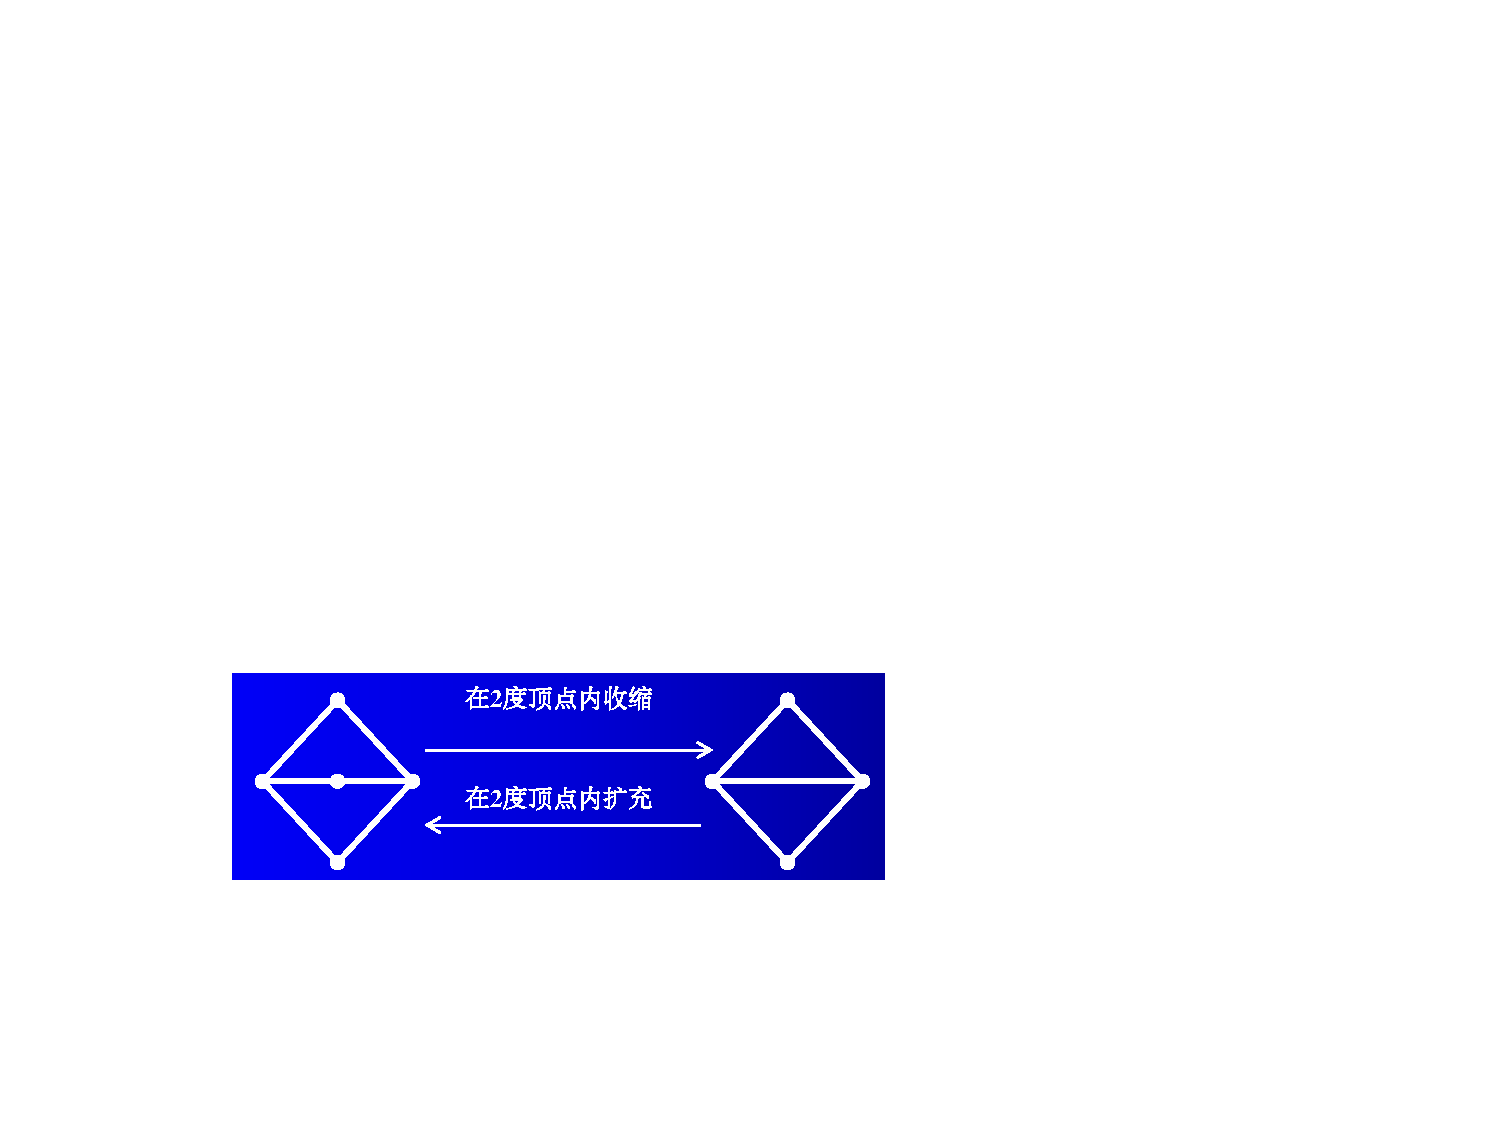
\includegraphics[scale=1.0]{image/CH6_tongpei.pdf}  
	%\caption{信息包结构} 
	\label{figkkjj1ik}  
\end{figure}

\begin{theorem}[库拉托斯基]
\colorbox{yellow}{图$G$是可平面的,当且仅当
它不含$K_5$和$K_{3,3}$同胚的子图}.
\end{theorem}

\begin{definition}
	给定图$G$, 去掉G中的环,用单边代替平行边而
	得到的图称为$G$的\colorbox{yellow}{\textcolor{red}{基础简单图}}.
\end{definition}
\begin{theorem}
	\begin{enumerate}
		\item 图$G$是可平面的当且仅当它的基础简单图
		是可平面的;
		\item 图$G$是可平面图当且仅当$G$的每个块是可平面图.
	\end{enumerate}
\end{theorem}


\begin{definition}
设$uv$是简单图$G$的一条边. 去掉该边,重合其
端点,再删去由此产生的环和平行边. 这一过程称为图
$G$的初等收缩或图的边收缩运算
\end{definition}
\begin{theorem}[瓦格纳]
	\colorbox{yellow}{简单图$G$是可平面图当且仅当它
	不含有可收缩到$K_5\mbox{或}K_{3,3}$的子图}.
\end{theorem}
\begin{note}
	彼得森图是不可平面图.
\end{note}
\begin{theorem}
	每一个至少有9个顶点的简单可平面图的补图是不可平
	面的,而9是这个数目中的最小的一个.
\end{theorem}
